%%% The main file. It contains definitions of basic parameters and includes all other parts.

%% Settings for single-side (simplex) printing
% Margins: left 40mm, right 25mm, top and bottom 25mm
% (but beware, LaTeX adds 1in implicitly)
\documentclass[12pt,a4paper]{report}
\setlength\textwidth{145mm}
\setlength\textheight{247mm}
\setlength\oddsidemargin{15mm}
\setlength\evensidemargin{15mm}
\setlength\topmargin{0mm}
\setlength\headsep{0mm}
\setlength\headheight{0mm}
% \openright makes the following text appear on a right-hand page
\let\openright=\clearpage

%% Settings for two-sided (duplex) printing
% \documentclass[12pt,a4paper,twoside,openright]{report}
% \setlength\textwidth{145mm}
% \setlength\textheight{247mm}
% \setlength\oddsidemargin{14.2mm}
% \setlength\evensidemargin{0mm}
% \setlength\topmargin{0mm}
% \setlength\headsep{0mm}
% \setlength\headheight{0mm}
% \let\openright=\cleardoublepage

%% Character encoding: usually latin2, cp1250 or utf8:
\usepackage[utf8]{inputenc}

%% Further useful packages (included in most LaTeX distributions)
\usepackage{amsmath}        % extensions for typesetting of math
\usepackage{amsfonts}       % math fonts
\usepackage{amsthm}         % theorems, definitions, etc.
\usepackage{bbding}         % various symbols (squares, asterisks, scissors, ...)
\usepackage{bm}             % boldface symbols (\bm)
\usepackage{graphicx}       % embedding of pictures
\usepackage{fancyvrb}       % improved verbatim environment
\usepackage{natbib}         % citation style AUTHOR (YEAR), or AUTHOR [NUMBER]
\usepackage[nottoc]{tocbibind} % makes sure that bibliography and the lists
			    % of figures/tables are included in the table
			    % of contents
\usepackage{dcolumn}        % improved alignment of table columns
\usepackage{booktabs}       % improved horizontal lines in tables
\usepackage{paralist}       % improved enumerate and itemize
\usepackage[usenames]{xcolor}  % typesetting in color
\usepackage{tocloft}        % for \cftchapnumwidth
\usepackage{amssymb}        % for \varnothing
\usepackage{hyphenat}       % for \hyp
\usepackage{float}          % for {figure}[H]
\usepackage{enumerate}      % for {enumerate}[(a)]
\usepackage[framemethod=default]{mdframed} % for {mymdframed}

%%% Basic information on the thesis

% Thesis title in English (exactly as in the formal assignment)
\def\ThesisTitle{Solving Endgames in Large \\ Imperfect-Information Games \\ such as Poker}

% Author of the thesis
\def\ThesisAuthor{Bc.~Karel Ha}

% Year when the thesis is submitted
\def\YearSubmitted{2016}

% Name of the department or institute, where the work was officially assigned
% (according to the Organizational Structure of MFF UK in English,
% or a full name of a department outside MFF)
\def\Department{Department of Applied Mathematics}

% Is it a department (katedra), or an institute (ústav)?
\def\DeptType{Department}

% Thesis supervisor: name, surname and titles
\def\Supervisor{Doc.~Mgr.~Milan Hladík, Ph.D.}

% Supervisor's department (again according to Organizational structure of MFF)
\def\SupervisorsDepartment{Department of Applied Mathematics}

% Study programme and specialization
\def\StudyProgramme{Computer Science}
\def\StudyBranch{Discrete~Models~\&~Algorithms}

% An optional dedication: you can thank whomever you wish (your supervisor,
% consultant, a person who lent the software, etc.)
\def\Dedication{%
  \todo
  %\begin{itemize}
  %  \item Nyx
  %  \item Milan Hladik
  %  \item parents
  %  \item CERN (hostels, library, facility)
  %\end{itemize}
}

% Abstract (recommended length around 80-200 words; this is not a copy of your thesis assignment!)
\def\Abstract{%
  \todo
}

% 3 to 5 keywords (recommended), each enclosed in curly braces
\def\Keywords{%
  {algorithmic game theory}, {imperfect-information games}, {Nash equilibrium},
  {subgame}, {endgame}, {counterfactual regret minimization}, {poker}
}

%% The hyperref package for clickable links in PDF and also for storing
%% metadata to PDF (including the table of contents).
\usepackage[pdftex,unicode]{hyperref}   % Must follow all other packages
\hypersetup{breaklinks=true}
\hypersetup{pdftitle={\ThesisTitle}}
\hypersetup{pdfauthor={\ThesisAuthor}}
\hypersetup{pdfkeywords=\Keywords}
\hypersetup{urlcolor=blue}

% Definitions of macros (see description inside)
%%% This file contains definitions of various useful macros and environments %%%
%%% Please add more macros here instead of cluttering other files with them. %%%

%%% Minor tweaks of style

% These macros employ a little dirty trick to convince LaTeX to typeset
% chapter headings sanely, without lots of empty space above them.
% Feel free to ignore.
\makeatletter
\def\@makechapterhead#1{
  {\parindent \z@ \raggedright \normalfont
   \Huge\bfseries \thechapter. #1
   \par\nobreak
   \vskip 20\p@
}}
\def\@makeschapterhead#1{
  {\parindent \z@ \raggedright \normalfont
   \Huge\bfseries #1
   \par\nobreak
   \vskip 20\p@
}}
\makeatother

% This macro defines a chapter, which is not numbered, but is included
% in the table of contents.
\def\chapwithtoc#1{
\chapter*{#1}
\addcontentsline{toc}{chapter}{#1}
}

% Draw black "slugs" whenever a line overflows, so that we can spot it easily.
\overfullrule=1mm

%%% Macros for definitions, theorems, claims, examples, ... (requires amsthm package)

\theoremstyle{plain}
\newtheorem{thm}{Theorem}
\newtheorem{lemma}[thm]{Lemma}
\newtheorem{claim}[thm]{Claim}

\theoremstyle{definition}
\newtheorem{defn}{Definition}

\theoremstyle{remark}
\newtheorem*{cor}{Corollary}
\newtheorem*{rem}{Remark}
\newtheorem*{example}{Example}

%%% An environment for proofs

%%% FIXME %%% \newenvironment{proof}{
%%% FIXME %%%   \par\medskip\noindent
%%% FIXME %%%   \textit{Proof}.
%%% FIXME %%% }{
%%% FIXME %%% \newline
%%% FIXME %%% \rightline{$\square$}  % or \SquareCastShadowBottomRight from bbding package
%%% FIXME %%% }

%%% An environment for typesetting of program code and input/output
%%% of programs. (Requires the fancyvrb package -- fancy verbatim.)

\DefineVerbatimEnvironment{code}{Verbatim}{fontsize=\small, frame=single}

%%% The field of all real and natural numbers
\newcommand{\R}{\mathbb{R}}
\newcommand{\N}{\mathbb{N}}

%%% Useful operators for statistics and probability
\DeclareMathOperator{\pr}{\textsf{P}}
\DeclareMathOperator{\E}{\textsf{E}\,}
\DeclareMathOperator{\var}{\textrm{var}}
\DeclareMathOperator{\sd}{\textrm{sd}}

%%% Transposition of a vector/matrix
\newcommand{\T}[1]{#1^\top}

%%% Various math goodies
\newcommand{\goto}{\rightarrow}
\newcommand{\gotop}{\stackrel{P}{\longrightarrow}}
\newcommand{\maon}[1]{o(n^{#1})}
\newcommand{\abs}[1]{\left|{#1}\right|}
\newcommand{\dint}{\int_0^\tau\!\!\int_0^\tau}
\newcommand{\isqr}[1]{\frac{1}{\sqrt{#1}}}

%%% Various table goodies
\newcommand{\pulrad}[1]{\raisebox{1.5ex}[0pt]{#1}}
\newcommand{\mc}[1]{\multicolumn{1}{c}{#1}}

%%%%%%%%%%%%%%%%%%%%%%%%%%%%%%%%%%%%%%%%%%%%%%
% The following section was added by Karel Ha.

% http://tex.stackexchange.com/questions/211414/chapter-0-roman-numerals
\newcommand{\ZeroAlph}[1]{% 0 + \Alph
  \ifcase\value{#1}\relax 0% Chapter 0
  \else\Alph{#1}\fi}% All other chapters
\renewcommand{\thechapter}{\ZeroAlph{chapter}}

% http://tex.stackexchange.com/questions/94464/note-environment-with-mdframed
\global\mdfdefinestyle{exampledefault}{%
  linecolor=lightgray,linewidth=1pt,%
  leftmargin=1cm,rightmargin=1cm,
}
\newenvironment{mymdframed}[1]{%
  \mdfsetup{%
    frametitle={\colorbox{white}{\,#1\,}},
    frametitleaboveskip=-\ht\strutbox,
    frametitlealignment=\raggedright
  }%
  \begin{mdframed}[style=exampledefault]
  }
  {%
  \end{mdframed}
}
\newcommand{\note}[1]{
  \begin{mymdframed}{Note}
    #1
  \end{mymdframed}
}


% mezera v Table of Contents před číslem kapitoly
\renewcommand*\cftchapnumwidth{2.2em}
\renewcommand*\cftsecnumwidth{2.6em}
\def\labelitemi{$\spadesuit$}
\def\labelitemii{$\diamondsuit$}

\newcommand{\HRule}{\rule{\linewidth}{0.5mm}}
\newcommand{\todo}{\textbf{\underline{TODO}}}
\renewcommand{\emptyset}{\varnothing}
\newcommand{\braces}[1]{ \left\{ #1 \right\} }
\newcommand{\I}{\mathcal{I}}
\newcommand{\Mueller}{M\"{u}ller}
\newcommand{\Zurich}{Z\"{u}rich}
\newcommand{\captionWithCite}[2]{ \caption[#1]{#1~(\cite{#2})} }

% black Chess pieces: http://tex.stackexchange.com/questions/150041/how-to-display-black-Chess-pieces-within-normal-text-with-Chessfss?rq=1
\newcommand{\pawnB}[1][1.3ex]{%
  \adjustbox{Trim=4.3pt 2.6pt 4.3pt 0pt,width=#1,margin=0.2ex 0ex 0.2ex 0ex}{\BlackPawnOnWhite}%
}%
\newcommand{\rookB}[1][1.58ex]{%
  \adjustbox{Trim=3.2pt 2.2pt 3.2pt 0pt,width=#1,raise=0ex,margin=0.1ex 0ex 0.1ex 0ex}{\BlackRookOnWhite}%
}%
\newcommand{\knightB}[1][1.85ex]{%
  \adjustbox{Trim=2.3pt 2.35pt 2.5pt 0pt,width=#1,raise=-0.03ex,margin=0.14ex 0ex 0.14ex 0ex}{\BlackKnightOnWhite}%
}%
\newcommand{\bishopB}[1][1.79ex]{%
  \adjustbox{Trim=2.3pt 2pt 2.3pt 0pt,width=#1,raise=-0.12ex,margin=0.1ex 0ex 0.1ex 0ex}{\BlackBishopOnWhite}%
}%
\newcommand{\queenB}[1][2.05ex]{%
  \adjustbox{Trim=1.2pt 2.2pt 1.2pt 0pt,width=#1,raise=-0.08ex,margin=0.1ex 0ex 0.1ex 0ex}{\BlackQueenOnWhite}%
}%
\newcommand{\kingB}[1][1.95ex]{%
  \adjustbox{Trim=2pt 2pt 2pt 0pt,width=#1,raise=-0.06ex,margin=0.13ex 0ex 0.13ex 0ex}{\BlackKingOnWhite}%
}%

\setlength{\epigraphwidth}{0.6\textwidth}
\renewcommand{\textflush}{flushepinormal} % justified text of epigraphs
\let\oldepigraph\epigraph
\renewcommand{\epigraph}[2]{\oldepigraph{#1}{#2}\noindent\ignorespaces}

\def\codeText#1{\texttt{#1}}

\renewcommand\qedsymbol{$\blacksquare$}
\newcommand{\lv}{\left\vert}
\newcommand{\rv}{\right\vert}
\DeclareMathOperator*{\argmin}{arg\,min}
\DeclareMathOperator*{\argmax}{arg\,max}

\hyphenation{
  e-qui-li-brium
  im-per-fect
  in-for-ma-tion
  end-game
  end-games
  da-ta-ba-se
  back-pro-pa-ga-te
  back-pro-pa-ga-ted
  ex-ten-si-ve
}
%%%%%%%%%%%%%%%%%%%%%%%%%%%%%%%%%%%%%%%%%%%%%%


% Title page and various mandatory informational pages
\begin{document}
%%% Title page of the thesis and other mandatory pages

%%% Title page of the thesis

\pagestyle{empty}
\hypersetup{pageanchor=false}
\begin{center}

\centerline{\mbox{
\includegraphics[width=166mm]{../img/logo-en.pdf}}}

\vspace{-8mm}
\vfill

{\bf\Large MASTER THESIS}

\vfill

{\LARGE\ThesisAuthor}

\vspace{15mm}

\HRule \\[0.6cm]
{\LARGE\bfseries\ThesisTitle}
\HRule \\[1.5cm]

\vfill

\Department

\vfill

\begin{tabular}{rl}

Supervisor of the master thesis: & \Supervisor \\
\noalign{\vspace{2mm}}
Study programme: & \StudyProgramme \\
\noalign{\vspace{2mm}}
Study branch: & \StudyBranch \\
\end{tabular}

\vfill

% Zde doplňte rok
Prague \YearSubmitted

\end{center}

\newpage

%%% Here should be a bound sheet included -- a signed copy of the "master
%%% thesis assignment". This assignment is NOT a part of the electronic
%%% version of the thesis. DO NOT SCAN.

%%% A page with a solemn declaration to the master thesis

\openright
\hypersetup{pageanchor=true}
\pagestyle{plain}
\pagenumbering{roman}
\vglue 0pt plus 1fill

\noindent
I declare that I carried out this master thesis independently, and only with the cited
sources, literature and other professional sources.

\medskip\noindent
I understand that my work relates to the rights and obligations under the Act No.~121/2000 Sb.,
the Copyright Act, as amended, in particular the fact that the Charles
University has the right to conclude a license agreement on the use of this
work as a school work pursuant to Section 60 subsection 1 of the Copyright Act.

\vspace{10mm}

\hbox{\hbox to 0.5\hsize{%
In ........ date ............	% FIXME!
\hss}\hbox to 0.5\hsize{%
signature of the author
\hss}}

\vspace{20mm}
\newpage

%%% Mandatory information page of the thesis

\openright

\vbox to 0.5\vsize{
\setlength\parindent{0mm}
\setlength\parskip{5mm}

Title:
{\let\\=\relax \ThesisTitle}

Author:
\ThesisAuthor

\DeptType:
\Department

Supervisor:
\Supervisor, \SupervisorsDepartment

Abstract:
\Abstract

Keywords:
\Keywords

\vss}

\newpage

%%% Dedication

\openright

\noindent
\Dedication

\newpage

\openright
\pagestyle{plain}
\pagenumbering{arabic}
\setcounter{page}{1}


%%% A page with automatically generated table of contents of the master thesis

\tableofcontents

%%% Each chapter is kept in a separate file
\setcounter{chapter}{-1}            % start from chapter 0
\chapter*{Introduction}
\addcontentsline{toc}{chapter}{Introduction}


\chapter{Background, Definitions and Notations}
\epigraph{
  I can't go to a~restaurant and order food because I keep looking at the fonts on~the menu.
}{Donald Ervin Knuth}

\section{General Game Theory}

\subsection{What Is Game Theory?}

The field of Game Theory deals with interactions or conflicts between $2$ or more agents.
\todo

A~\emph{(simultaneous move) game} consists of: \todo
\begin{itemize}
  \item set $P$ of players $\braces{1, 2, \cdots, n}$
  \item actions
  \item payoffs
\end{itemize}

There are additional concepts related to games such as: \todo
\begin{itemize}
  \item \emph{strategy}
  \item \emph{dominant strategy}
  \item \emph{best response}
  \item \emph{pure Nash equilibrium}
  \item \emph{mixed strategy}
  \item \emph{(mixed) Nash equilibrium}
  \item \emph{correlated equilibrium}
\end{itemize}

A~\emph{game with turns} has:
\begin{itemize}
  \item \todo
\end{itemize}

\subsection{Representation of Games}

\todo
\begin{itemize}
  \item standard (matrix) form
  \item compactly represented game
\end{itemize}

There will be other kinds of representation for extensive form games (see Subsection~\ref{ssec:extensive-form}).

\subsection{Standard Examples}

\todo %Describe the games and how the game-theoretic definitions from above look like in these examples

\begin{itemize}
  \item{Rock-paper-scissors}
  \item{Chess}
  \item{Poker}
\end{itemize}

\section{Combinatorial Game Theory}
\label{sec:CGT}

\todo

\section{The Game of Go}
\label{sec:Go}

\subsection{Rules}

\emph{Black} and \emph{White} place pieces (\emph{stones}) on the unoccupied intersections (\emph{points}) of a~\emph{board} with a~$19\times19$ grid of~lines.
Players take turns, Black moves first.
There are only 2 basic rules of Go:
\begin{description}
  \item [The rule of liberty]
    Every stone remaining on the board must have at least one open point (an~intersection, called a~\emph{liberty}) directly next to it (up, down, left, or right), or must be part of a~connected group that has at least one such liberty next to it.
    \begin{figure}[H]
      \centering
      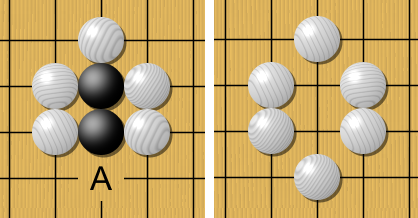
\includegraphics[width=.5\textwidth]{../img/Go_rule_of_liberty.png}
      \caption{The rule of liberty}
      \label{fig:Go-rule-liberty}
    \end{figure}

    Stones or groups of stones which lose their last liberty are removed from the board.

  \item [The ``ko'' rule]
    The stones on the board must never repeat a~previous position of~stones.
    This is to prevent unending cycles.
    \begin{figure}[H]
      \centering
      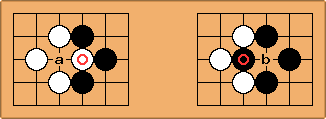
\includegraphics[width=.5\textwidth]{../img/Go_ko_rule.png}
      \caption{The ``ko'' rule}
      \label{fig:Go-Ko-rule}
    \end{figure}

\end{description}

\subsection{Scoring, Ranks and Handicaps}

There are several \textbf{scoring rules} to determine the winner of a~game.
In the match of~AlphaGo against Lee Sedol,%
\footnote{See Chapter~\ref{ch:AlphaGo}.}
the \emph{area scoring} was used.
Under area scoring system, player's score is:
\begin{itemize}
  \item the number of stones that the player has on the board
  \item plus the number of~empty intersections surrounded by that player's stones
  \item plus \emph{komi(dashi)} points%
    \footnote{a~compensation for the first move advantage of~the Black player}
    for the White player
\end{itemize}

\emph{Elo rating} can be used to denote players' \textbf{ranks}.
Alternatively, \emph{kyu/dan} (in~Japanese) or \emph{gup/dan} (in~Korean) system is also vastly popular:
\begin{figure}[H]
  \centering
  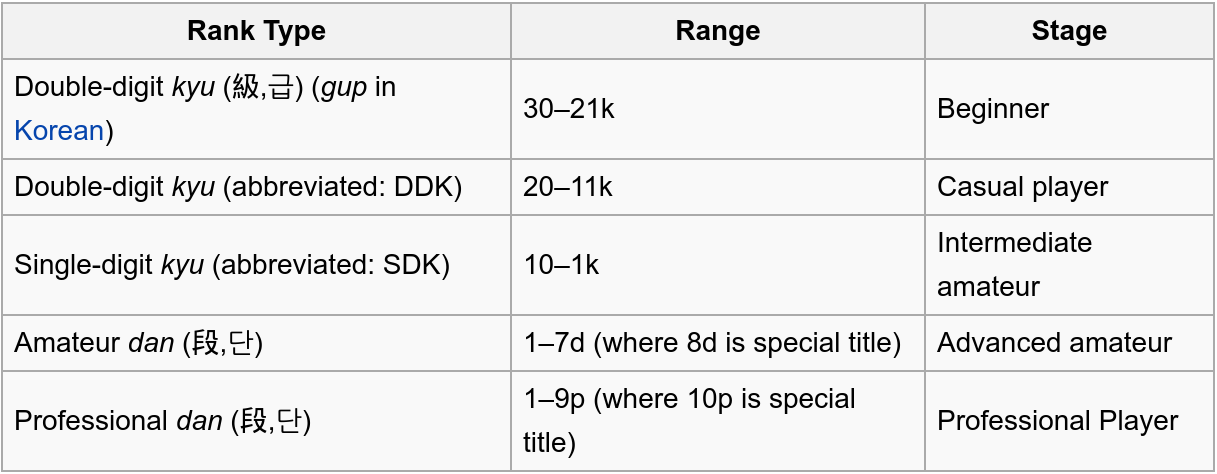
\includegraphics[width=.8\textwidth]{../img/Go_kyu_dan.png}
  \caption{Kyu/Gup and Dan ranks}
  \label{fig:Go-ranks}
\end{figure}

\textbf{Handicap} system is used to even up differences in ranks:
Black can place 1 or more stones in advance as a~compensation for White's greater strength.

\section{Algorithmic Game Theory}

\subsection{What Is Algorithmic Game Theory?}
One of the classic textbook is the extensive \emph{Algorithmic Game Theory} (\cite{AGT07}).
\todo

\subsection{Examples from Algorithmic Game Theory}

The following games capture various game-theoretic properties and the ``real-life'' counterparts of these games in the fields such as networking, economy etc.
The examples and figures are taken from \emph{Algorithmic Game Theory} (\cite{AGT07}).

\newcommand{\widthratio}{0.3}
\begin{itemize}
  \item \emph{Prisoner's dilemma} \todo
    \begin{figure}[H]
      \centering
      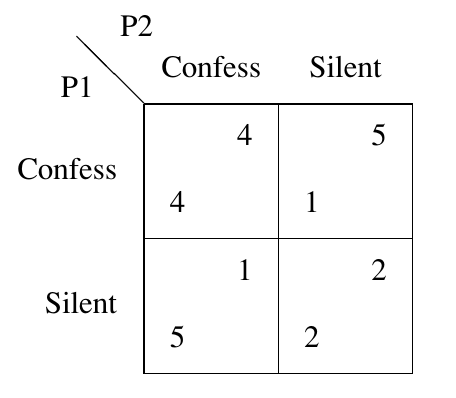
\includegraphics[width=\widthratio\paperwidth]{../img/prisoner.png}
      \caption{Prisoner's dilemma}
      \label{fig:prisoner}
    \end{figure}

    \begin{figure}[H]
      \centering
      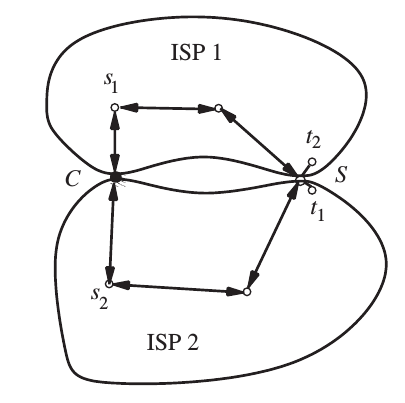
\includegraphics[width=\widthratio\paperwidth]{../img/isp.png}
      \caption{ISP routing game}
      \label{fig:isp-routing}
    \end{figure}


  \item \emph{Pollution game} is a multi-player version of Prisoner's dilemma \todo

  \item An~example of a~coordination game is the \emph{Battle of sexes}.

    \begin{figure}[H]
      \centering
      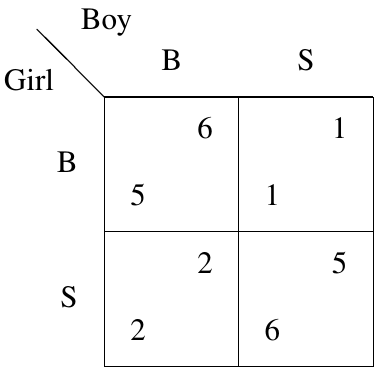
\includegraphics[width=\widthratio\paperwidth]{../img/battle-of-sexes.png}
      \caption{Battle of sexes}
      \label{fig:battle-of-sexes}
    \end{figure}

  \item Another coordination game is the \emph{Routing congestion game}, taken from the world of networking

    \begin{figure}[H]
      \centering
      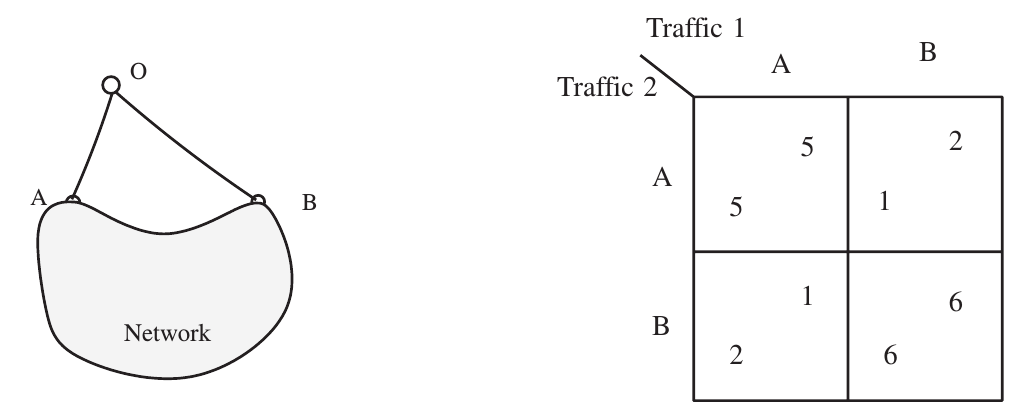
\includegraphics[width=0.65\paperwidth]{../img/routing-congestion-game.png}
      \caption{Routing congestion game}
      \label{fig:routing-congestion}
    \end{figure}

  \item \emph{Matching pennies} can be considered as a $2$-choice reduction of Rock-paper-scissors.

    \begin{figure}[H]
      \centering
      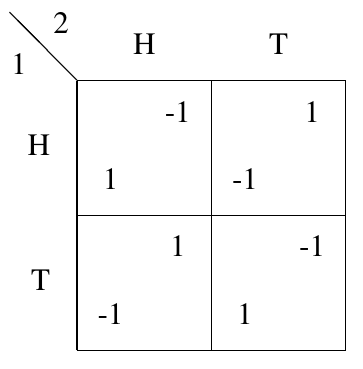
\includegraphics[width=\widthratio\paperwidth]{../img/matching-pennies.png}
      \caption{Matching pennies}
      \label{fig:matching-pennies}
    \end{figure}

  \item \emph{Pricing game} is an~example of a~game without a~(mixed) Nash equilibrium.

    \begin{figure}[H]
      \centering
      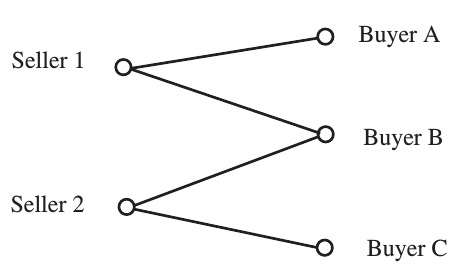
\includegraphics[width=\widthratio\paperwidth]{../img/pricing-game.png}
      \caption{Pricing game}
      \label{fig:pricing-game}
    \end{figure}

  \item \emph{Traffic light}

    \begin{figure}[H]
      \centering
      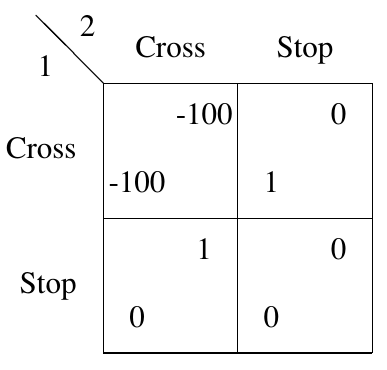
\includegraphics[width=\widthratio\paperwidth]{../img/traffic-light.png}
      \caption{Traffic light}
      \label{fig:traffic-light}
    \end{figure}

  \item \emph{Ultimatum game}
\end{itemize}

\subsection{Extensive Form}
\label{ssec:extensive-form}

An \emph{extensive-form game} consists of

\begin{itemize}
  \item a finite set of \emph{players} $P$,
  \item a finite set $H$ of all possible \emph{histories},
    \begin{itemize}
      \item Each history consists of individual \emph{actions}.
      \item $h \sqsubseteq h'$ denotes that history~$h$ is a~prefix of $h'$.
      \item $\emptyset \in H$ and $h' \in H \land h \sqsubseteq h' \implies h \in H$
      \item Set $Z \subseteq H$ is the set of \emph{terminal histories}, i.e. histories that are not prefixes of any other histories.
    \end{itemize}
  \item the set of available actions $A(h) = \braces{a: (h, a) \in H}$ for every node $h \in H \setminus Z$,
  \item a~function $P()$ assigning an~\emph{acting player} to each $h \in H \setminus Z$.
    The acting players are taken from the set $P \cup \braces{c}$, where $c$ is the \textbf{c}hance player (e.~g. a~dice, the card dealer, the nature etc.).
    Thus, $P(h) \in P \cup \braces{c}$ for any $h \in H \setminus Z$.
  \item a~function $f_c$ determining the probability measure over actions $A(h)$ for nodes $h$ with $p(h) = c$, the nodes of the chance player.
  \item The partition $\I_i$ of nodes $\braces{h \in H: p(h) = i}$ is called the \emph{information partition} of player~$i$.
    Its element $I \in \I_i$ is an \emph{information set} of player~$i$ and $I(h) \in \I_i$ (with $p(h) = i$) denotes the information set containing $h$.

    An information set represents grouping of histories that are indistinguishable from $i$'s point of view.
    In the game of poker, for example, this might be because of hidden cards of opponents.
  \item a \emph{utility function} $u_i\colon Z \goto \R$,
\end{itemize}

There are further notions related to any extensive-form game:

\begin{itemize}
  \item \emph{Strategy}~$\sigma_i$ of (non-chance) player~$i$ determines a~probability distribution over $A(I)$ at every $I \in \I_i$.
    Thus $\pi ^\sigma (I, a)$ is the probability of action $a$ at the information set~$I$.
    $\Sigma_i$ denotes the set of all possible strategies for player~$i$.
  \item A~\emph{strategy profile} is a~vector of all (non-chance) players' strategies denoted by $\sigma = (\sigma_1, \sigma_2, \ldots, \sigma_ {\abs{P}})$.
    The set of all such possible strategy profiles is denoted by $\Sigma$.
    Hence, it is the Cartesian product $\Sigma = \prod\limits _{i \in P} \Sigma_i$.
  \item We use the Greek letter $\pi$ to evaluate the probability corresponding to a~profile~$\sigma$:
    \[\pi ^\sigma(h) = \prod _{i \in P \cup \braces{c}} \pi _i ^\sigma (h)\]
    
  \item The probability $\pi _{-i} ^\sigma (h)$ (or sometimes just briefly $\pi _{-i} (h)$) is the product of~all players' contribution, except for the one of player~$i$:
    \[\pi _{-i} ^\sigma(h) = \prod _{j \in P \setminus \braces{i} \cup \braces{c}} \pi _j ^\sigma (h)\]
    
  \item $\sigma | _{I \goto a}$ denotes the strategy identical to $\sigma$ with the only one exception:
    the action~$a$ is always played at the information set~$I$.
  \item Given the strategic profile $\sigma$, the \emph{expected utility}~$u_i (\sigma)$ for player~$i$ is defined as:
    \[ u_i (\sigma) = \sum _{z \in Z} \pi ^\sigma (z) u_i(z)\]

  \item A~\emph{best response} $BR _i (\sigma _{-i})$ (or briefly $BR _i (\sigma)$) of player $i$ for given $\sigma _{-p}$ is such a~strategy $\sigma _i \in \Sigma _i$ that maximizes player's expected utility against others:
    \[ u_i (\sigma) = \max _{\sigma'_i \in \Sigma_i} u_i ((\sigma'_i, \sigma_{-i})) \]

  \item A~\emph{Nash equilibrium} (in the context of extensive-form games) is a~strategy profile $\sigma$ such that no player~$i \in P$ has any incentive to deviate from his strategy.
    In other words, all players are playing best responses against each other:
    \[ \forall i \in P\colon u_i (\sigma) = \max _{\sigma'_i \in \Sigma_i} u_i ((\sigma'_i, \sigma_{-i})) \]

  \item The \emph{counterfactual value} $v _i ^\sigma (I)$ is the expected utility provided that the information set $I$ is reached and all players play according to strategy $\sigma$ with exception of player~$i$, who plays to reach $I$:
    \[ v _i ^\sigma (I) = \sum\limits _{h \in I, \; h' \in Z}
      \frac
      {\pi _{-i} ^\sigma(h) \pi ^\sigma(h,h') u_i(h')}
      {\pi _{-i} ^\sigma (I)} \]

  \item A~\emph{counterfactual best response} $CBR _i (\sigma _{-i})$ (or briefly $CBR _i (\sigma)$) of player~$i$ is a~strategy maximizing the counterfactual value at each information set $I \in \I _i$:
    \[ \pi ^\sigma (I, a) \geq 0
      \; \Longleftrightarrow \;
      v _i ^\sigma (I, a) = \max _{a' \in A(I)} v _i ^\sigma (I, a') \]

    Note that $CBR _i (\sigma)$ is always a best response $BR _i (\sigma)$, but the reverse implication does not need to hold:
    a~best response $\sigma$ can select an~arbitrary action in an~unreachable information set $I$ (the one where $\pi ^\sigma (I) = 0$).
    Such best responses are in general not counterfactual best responses.

  \item For the sake of notation's simplicity, we will define \emph{counterfactual best response value} as the counterfactual value for the strategy, where player $i$ plays according $CBR _i (\sigma _{-i})$ rather than the original $\sigma$.
    Formally, it is
    \[ CBV _i ^\sigma (I) = v _i ^{(\sigma _{-i}, CBR _i (\sigma _{-i} ))} (I) \]

\end{itemize}

There may be various properties for extensive-form games:

\begin{itemize}
  \item being \emph{two-player}
  \item having \emph{perfect recall}: any two states from the same information set $I \in \I _i$ share the same history of past actions and player $i$'s information sets.

    In other words, at any stage of the game no player can forget what happened so far:
    neither actions taken nor the information sets reached.
  \item being \emph{zero-sum}: For any $\sigma \in \Sigma$ we have $\sum _{i \in P} u _i (\sigma) = 0$.
\end{itemize}

\subsection{Sequence Form}

\section{Methods of~Solution}

\subsection{Linear Programming}
{
  \setlength{\epigraphwidth}{0.65\textwidth}
  \epigraph{
    If you optimize everything, you will always be unhappy.
  }{Donald Ervin Knuth}
}

\subsection{Learning}

\section{Subgames (Endgames)}

So far, the information sets have grouped only those states where the player was the acting player.
For the purposes of the subgame, it is also necessary to include the states that are indistinguishable from the point of view of other players.
Therefore, we define the \emph{augmented information sets} (\cite{BurchJohansonBowling13}):

\begin{itemize}
  \item For any player $i \in P$, let $H_i(h)$ be the sequence of player $i$'s information sets reached by player $i$ on the path to $h$, and the actions taken by player~$i$.
  \item An~\emph{augmented information set} $I_i(h)$ is defined by the following characterization:
    for any two states $h, h' \in H$, we have that 
    \[ I_i (h) = I_i (h') \; \Longleftrightarrow \; H_i (h) = H_i (h') \]
\end{itemize}

At this point, we may finally define the notion of a~\emph{subgame}:

\begin{itemize}
  \item An~(imperfect information) \emph{subgame} is a~forest of trees, closed under both the descendant relation and membership within augmented information sets for any player (\cite{BurchJohansonBowling13}).
\end{itemize}

\subsection{Previous Works}

\chapter{Background, Definitions and Notations}

The field of Game Theory deals with interactions or conflicts between $2$ or more agents.
\todo

\section{General Game Theory}

\begin{itemize}
  \item players
  \item actions
  \item payoffs
  \item \emph{Nash equilibrium}
  \item \emph{best response}
\end{itemize}

\subsection{Extensive form}

An \emph{extensive-form game} consists of

\begin{itemize}
  \item a finite set of \emph{players} $P$,
  \item a finite set $H$ of all possible \emph{histories},
    \begin{itemize}
      \item Each history consists of individual \emph{actions}.
      \item $h \sqsubseteq h'$ denotes that history~$h$ is a~prefix of $h'$.
      \item $\emptyset \in H$ and $h' \in H \land h \sqsubseteq h' \implies h \in H$
      \item Set $Z \subseteq H$ is the set of \emph{terminal histories}, i.e. histories that are not prefixes of any other histories.
    \end{itemize}
  \item the set of available actions $A(h) = \braces{a: (h, a) \in H}$ for every node $h \in H \setminus Z$,
  \item a~function $p$ assigning an~\emph{acting player} to each $h \in H \setminus Z$.
    The acting players are taken from the set $P \cup c$, where $c$ is the \textbf{c}hance player (e.~g. a~dice, the card dealer, the nature etc.).
  \item a~function $f_c$ determining the probability measure over actions $A(h)$ for nodes $h$ with $p(h) = c$, the nodes of the chance player.
  \item The partition $\I_i$ of nodes $\braces{h \in H: p(h) = i}$ is called the \emph{information partition} of player~$i$.
    Its element $I \in \I_i$ is an \emph{information set} of player~$i$.
    An information set represents grouping of histories that are indistinguishable from $i$'s point of view.
    In the game of poker, for example, this might be because of hidden cards of opponents.
  \item a \emph{utility function} $u_i\colon Z \goto \R$,
\end{itemize}

There are further notions related to any extensive-form game:

\begin{itemize}
  \item \emph{strategy}
  \item \emph{strategy profile}. $\Sigma$
  \item \emph{counterfactual value}
  \item \emph{counterfactual best response}
  \item \emph{counterfactual best response value}
\end{itemize}

There may be various properties, which an~extensive-form game can have.
Such a~game can:

\begin{itemize}
  \item be \emph{two-player}
  \item have \emph{perfect recall}
  \item be \emph{zero-sum}
\end{itemize}

\subsection{Sequence form}

\section{Methods of~solution}

\subsection{Linear programming}

\subsection{Learning}

\section{Subgames (endgames)}

\subsection{Previous works}

\chapter{Endgame Solving}

This chapter summarizes the approach, methods and results from the article ``Improving Performance in Imperfect\hyp{}Information games with Large State and Action Spaces by Solving Endgames''~\cite{GanzfriedSandholm13improving}.

\section{Motivation}

\section{Gadget game tree}

\section{Equivalent linear program}

\section{Experimental results}

\chapter{Endgame Solving}

This chapter summarizes the approach, methods and results from the article ``Improving Performance in Imperfect\hyp{}Information games with Large State and Action Spaces by Solving Endgames''~\cite{GanzfriedSandholm13improving}.

\section{Motivation}

\section{Gadget game tree}

\section{Equivalent linear program}

\section{Experimental results}

\chapter{CFR-D}

This chapter summarizes the approach, methods and results from the paper ``Solving Imperfect Information Games Using Decomposition'' (\cite{BurchJohansonBowling13}).

\section{Motivation}

\section{Gadget Game-Tree}

\section{Equivalent Linear Program}

\section{Experimental Results}

\chapter{Subgame Margin Maximization}

\section{Motivation}

\section{Subgame Margin}

\begin{defn}[Subgame margin]
\end{defn}

\begin{thm}[improvement is proportional to the subgame margin (and may be greater)]
  \todo
\end{thm}

\begin{proof}
  \todo
\end{proof}

\section{Equivalent Linear Program}

\section{Gadget Game}

\section{Experimental Results}

\chapter{Ideas for Future Work: Other Possible Objective Functions}
\epigraphLong{
  Raise your quality standards as~high as you can live with, avoid wasting your time on~routine problems, and always try to~work as~closely as~possible at~the boundary of~your abilities.
  Do this, because it is the only way of~discovering how that boundary should be moved forward.
}{Edsger Wybe Dijkstra}
\epigraphLong{
  The worst thing that can happen in a~democracy---as well as in an~individual's life---is to become cynical about the future and lose hope.
}{Hillary Diane Rodham Clinton}


\chapter*{Conclusion}
\addcontentsline{toc}{chapter}{Conclusion}
\epigraphLong{
  Everything that civilisation has to~offer is a~product of human intelligence;
  we cannot predict what we might achieve when this intelligence is magnified by~the tools that AI may provide, but the eradication of~war, disease, and poverty would be high on~anyone's list.
  Success in~creating AI would be the biggest event in~human history.
  Unfortunately, it might also be the last.
}{Stephen Hawking}
Perfect-information endgames can be solved by backward induction, where solutions to subgames are propagated up the game tree.
For the imperfect information, on~the other hand, endgames need to be adjusted in~order to account for information sets.
This gives rise to a~new definition of~an~(imperfect-information) \emph{subgame}.
As such, the definition does not directly allow to apply the same procedure as in~perfect-information endgames:
under even the simplest conditions of~the \acrlong{rps} game, a~na{\"i}ve endgame re-solution fails to form a~\acrlong{ne}.

This occurs because the opponent can change his behavior prior to the endgame.
Such an~exploitation power can be captured by~a~\emph{counterfactual value}:
a~hypothetical ``what-if'' value summarizing opponent's improvement, if he had changed his prior trunk strategy.

We used counterfactual values to define our own notion of~\emph{\acrlong{sm}}:
a~gap between the original and the new \acrlong{cbv}s.
We related the \acrshort{sm} to the exploitability against a~\acrlong{br}, and we proved the overall improvement rising from endgame improvement is proportional to the \acrshort{sm}.

Maximizing \acrshort{sm} is thus highly advisable.
That can be achieved either by solving a~variant of a~sequence-form \acrlong{lp}, or by applying an~iterative learning algorithm to a~\emph{gadget game}, an~equivalent ad-hoc \acrlong{efg}.
The latter approach offers greater benefits in~terms of~exploiting domain-specific knowledge and employing powerful learning algorithms such as \acrshort{cfr}, \acrshort{mccfr} or the~modern \cfrplus{} that we chose to solve our \emph{max-margin gadget}.

Finally, we experimentally compared the three contemporary approaches to solving endgames:
\begin{enumerate}[(i)]
  \item endgame solving (\cite{Ganzfried2015endgame})
  \item \acrshort{cfr-d} and decomposition (\cite{BurchJohansonBowling2014})
  \item our subgame-margin maximization (\cite{Moravcik2016refining})
\end{enumerate}
The results of~the experiments showed that (i) even produced a~worse \acrshort{sm}, leading to more exploitable subgame strategies;
and although the \acrshort{sm} of~(ii) increased over time, the improvement was not significant, as the method guarantees only the same (or comparable) quality, not the best one.
Since our (iii) was specially designed to maximize \acrshort{sm}s, it re-created the most robust (i.e., the least exploitable) subgame strategy.
We thus offer a~superior solution to treating subgames.


%%% Bibliography
%%% Bibliography (literature used as a source)
%%%
%%% We employ bibTeX to construct the bibliography. It processes
%%% citations in the text (e.g., the \cite{...} macro) and looks up
%%% relevant entries in the bibliography.bib file.
%%%
%%% The \bibliographystyle command selects, which style will be used
%%% for references from the text. The argument in curly brackets is
%%% the name of the corresponding style file (*.bst). Both styles
%%% mentioned in this template are included in LaTeX distributions.

\bibliographystyle{plainnat}    %% Author (year)
% \bibliographystyle{unsrt}     %% [number]

\renewcommand{\bibname}{Bibliography}

%%% Generate the bibliography. Beware that if you cited no works,
%%% the empty list will be omitted completely.

\bibliography{bibliography}

%%% If case you prefer to write the bibliography manually (without bibTeX),
%%% you can use the following. Please follow the ISO 690 standard and
%%% citation conventions of your field of research.

% \begin{thebibliography}{99}
%
% \bibitem{lamport94}
%   {\sc Lamport,} Leslie.
%   \emph{\LaTeX: A Document Preparation System}.
%   2nd edition.
%   Massachusetts: Addison Wesley, 1994.
%   ISBN 0-201-52983-1.
%
% \end{thebibliography}


%%% Figures used in the thesis (consider if this is needed)
\listoffigures

%%% Tables used in the thesis (consider if this is needed)
%%% In mathematical theses, it could be better to move the list of tables to the beginning of the thesis.
\listoftables

%%% Abbreviations used in the thesis, if any, including their explanation
%%% In mathematical theses, it could be better to move the list of abbreviations to the beginning of the thesis.
\chapwithtoc{List of Abbreviations}

%%% Attachments to the master thesis, if any. Each attachment must be
%%% referred to at least once from the text of the thesis. Attachments
%%% are numbered.
%%%
%%% The printed version should preferably contain attachments, which can be
%%% read (additional tables and charts, supplementary text, examples of
%%% program output, etc.). The electronic version is more suited for attachments
%%% which will likely be used in an electronic form rather than read (program
%%% source code, data files, interactive charts, etc.). Electronic attachments
%%% should be uploaded to SIS and optionally also included in the thesis on a~CD/DVD.
\chapwithtoc{Attachments}

\openright
\end{document}
